
% this file is called up by thesis.tex
% content in this file will be fed into the main document

%: ----------------------- introduction file header -----------------------
% the code below specifies where the figures are stored
\graphicspath{{2/figures/}}

\chapter{Context}
\label{chp:context}

% Goals of this chapter
% ------------
% State of MIR
% Reassessment of common practice
% Summary of findings
% Proposed solution -- deep learning
%   Deep architectures
%   Feature learning
% Previous work in MIR


\section{State of Affairs in MIR}



From its inception, many fundamental challenges in content-based music informatics, and more specifically those that focus on music audio signals, have received a considerable and sustained research effort from the community.
This area of study falls under the umbrella of perceptual AI, operating on the premise that if a human expert can experience some musical event from an audio signal, it should be possible to make a machine respond similarly.
As the field continues into its second decade, there are a growing number of resources that comprehensively review the state of the art in these music signal processing systems across a variety of different application areas  \cite{Klapuri2006,Casey2008,Mueller2011a}, including melody extraction, chord recognition, beat tracking, tempo estimation, instrument identification, music similarity, genre classification, and mood prediction, to name only a handful of the most prominent topics.

% Things aren't solved; why?
After years of diligent effort however, many well-worn problems in content-based MIR lack sufficiently ``good'' solutions, and thus in some sense remain unsolved.
Observing this larger research trajectory at a distance, it would seem progress is decelerating, if not altogether stalled.
For example, a review of recent MIREX\footnote{Music Information Retrieval Evaluation eXchange (MIREX): {http://www.music-ir.org/mirex/}} results motivates the conclusion quantitatively, as shown in Figure \ref{fig:mirex}.
The three most consistently evaluated tasks for more than the past half decade ---chord recognition, genre recognition, and mood estimation--- are each converging to performance plateaus below satisfactory levels.
Fitting an intentionally generous logarithmic model to the progress in chord estimation, for example, estimates that continued performance at this rate would eclipse 90\% in a little over a decade, and 95\% some twenty years after that; note that even this trajectory is quite unlikely, and for only this one specific problem (and dataset).
Attempts to extrapolate similar projections for the other two tasks are even less encouraging.
Furthermore, these ceilings are pervasive across many open problems in the discipline.
Though single-best accuracy over time is shown for these three specific tasks, a wider space of MIREX tasks exhibit similar, albeit more sparsely sampled, trends.
Recent research has additionally demonstrated that when state-of-the-art algorithms are employed in more realistic situations, i.e. larger datasets, performance degrades substantially \cite{BertinMahieux2012}.
In a complementary, if antagonizing, vein, others have begun to challenge the very notion that progress has even been made at all, due to issues of problem formulation and validity \cite{Sturm2013}.
Consequently, these observations have encouraged some to question the state of affairs in content-based MIR:
Does content \emph{really} matter, especially when human signals have proven to be more useful than those derived from the content itself \cite{Slaney2011}?
If so, what can be learned by analyzing recent approaches to content-based analysis \cite{Flexer2012}?
How might MIR challenges be better formalized and evaluated \cite{Sturm2014}?
And, are there other approaches to building computational systems to solve these problems \cite{Humphrey2012a}?

\begin{figure}
\begin{centering}
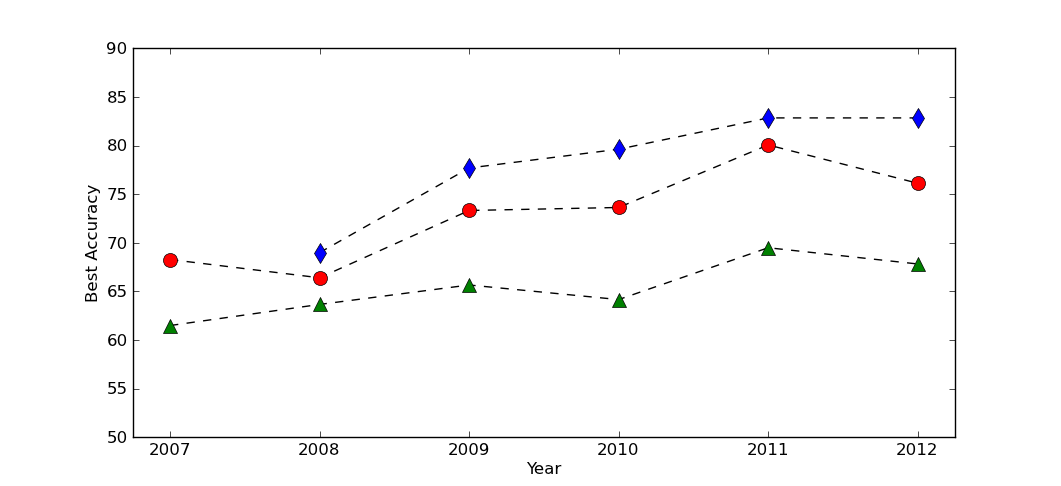
\includegraphics[width=\textwidth]{mirex2}
\caption{\emph{Losing Steam}: The best performing systems at MIREX since 2007 are plotted as a function of time for Chord Estimation (blue diamonds), Genre Recognition (red circles), and Mood Prediction (green triangles).}
\label{fig:mirex}
\end{centering}
\end{figure}

Acknowledging that content-based MIR is indeed valuable, this chapter is an attempt to answer the remainder of these questions.
Section \ref{sec:common} critically reviews conventional approaches to content-based analysis and identifies three major deficiencies of current systems: the sub-optimality of hand-designing features, the limitations of shallow architectures, and the short temporal scope of signal analysis.
Afterwards, Section \ref{sec:timeliness} discusses why it is critical for the MIR community to address these issues \emph{now}.



\section{Reassessing Common Practice in Content-based MIR}
\label{sec:common}

Despite a broad spectrum of application-specific problems, the vast majority of music signal processing systems adopt a common two-stage paradigm of feature extraction and semantic interpretation.
Leveraging substantial domain knowledge and a deep understanding of digital signal theory, researchers carefully architect signal processing systems to capture useful signal-level attributes, referred to as \emph{features}.
These signal features are then provided to a pattern recognition machine for the purposes of assigning semantic meaning to observations.
Crafting good features is a particularly challenging subproblem, and it is becoming standard practice amongst researchers to use precomputed features\footnote{Million Song Dataset} or off-the-shelf implementations\footnote{MIR Toolbox, Chroma Toolbox, MARSYAS, Echonest API}, focusing instead on increasingly more powerful pattern recognition machines to improve upon prior work.
Therefore, while early research mainly employed simple classification strategies such as nearest-neighbors or peak-picking, recent work makes extensive use of sophisticated and versatile techniques, e.g. Support Vector Machines \cite{Mandel2005}, Bayesian Networks \cite{Mauch2010a}, Conditional Random Fields \cite{Sumi2012}, and Variable-Length Markov Models \cite{Chordia2011}.

\begin{figure}
\begin{centering}
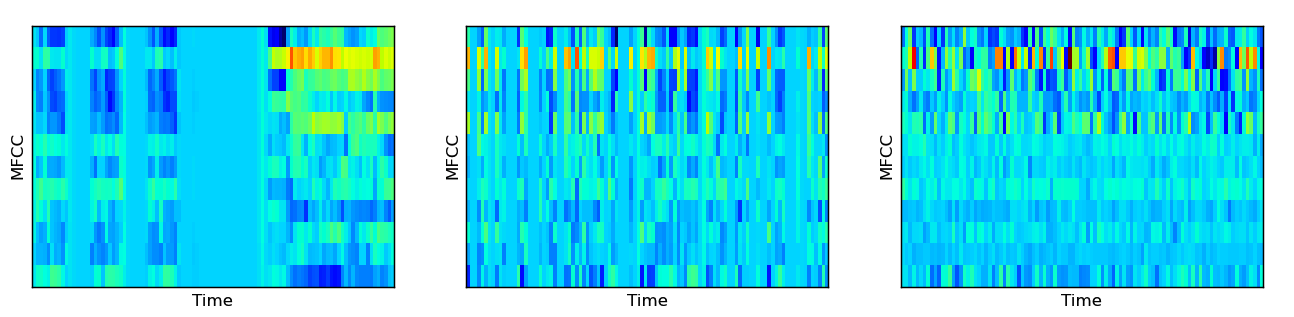
\includegraphics[width=\textwidth]{mtb_mfccs}
\caption{\emph{What story do your features tell?} Sequences of MFCCs are shown for a real music excerpt (left), a time-shuffled version of the same sequence (middle), and an arbitrarily generated sequence of the same shape (right). All three representations have equal mean and variance along the time axis, and could therefore be modeled by the exact same distribution.}
\label{fig:mfccs}
\end{centering}
\end{figure}

This trend of squeezing every bit of information from a stock feature representation is arguably questionable because the two-tier perspective hinges on the premise that \emph{features are fundamental}.
Data must be summarized in such a way that the degrees of freedom are informative for a particular task; features are said to be \emph{robust} when this is achieved, and \emph{noisy} when variance is misleading or uninformative.
The more robust a feature representation is, the simpler a pattern recognition machine needs to be, and vice versa.
It can be said that robust features \emph{generalize} by yielding accurate predictions of new data, while noisy features can lead to the opposite behavior, known as \emph{over-fitting} \cite{Bishop2006}.
The substantial emphasis traditionally placed on feature design demonstrates that the community implicitly agrees, but it is a point worth illustrating.
Consider the scenario presented in Figure \ref{fig:mfccs}.
The predominant approach to compute how similar two music signals sound is to model their Mel-Frequency Cepstral Coefficients (MFCCs) with a Gaussian Mixture Model (GMM) and compute some distance measure between them, e.g. KL-divergence, Earth mover's distance, etc. \cite{Berenzweig2004}.
Importantly though, representing these coefficients as a mixture of Gaussians reduces the observation to mean and variance statistics, discarding temporal structure.
Therefore, the three MFCC sequences shown ---a real excerpt, a shuffled version of it, and a randomly generated one--- are identical in the eyes of the model.
The audio that actually corresponds to these respective representations, however, will certainly not \emph{sound} similar to a human listener.

This bears a significant consequence: any ambiguity introduced or irrelevant variance left behind in the process of computing features must instead be overcome by the pattern recognition machine.
Previous research in chord recognition has explicitly shown that better features allow for simpler classifiers \cite{Cho2011}, and intuitively many have spent years steadily improving their respective feature extraction implementations \cite{Lyon2010,Mueller2011b}.
Moreover, there is ample evidence these various classification strategies work quite well on myriad problems and datasets \cite{Bishop2006}.
Therefore, underperforming content-based MIR systems are more likely the result of deficiencies in the feature representation than the classifier used to make sense of it.


It is particularly prudent then, to examine the assumptions and design decisions incorporated into feature extraction systems.
In music signal processing, audio feature extraction typically consists of a recombination of a small set of operations, as depicted in Figure \ref{fig:simplearch}: splitting the signal into independent short-time segments, referred to as blocks or frames; applying an affine transformation, generally interpreted as either a projection or filterbank; applying a non-linear function; and pooling across frequency or time.
Some of these operations can be, and often are, repeated in the process.
For example, MFCCs are computed by filtering a signal segment at multiple frequencies on a Mel-scale (affine transform), taking the logarithm (non-linearity), and applying the Discrete Cosine Transform (affine transformation).
Similarly, chroma features are produced by applying a constant-Q filterbank (affine transformation), taking the complex modulus of the coefficients (non-linearity), and summing across octaves (pooling).

\begin{figure}[t]
\begin{centering}
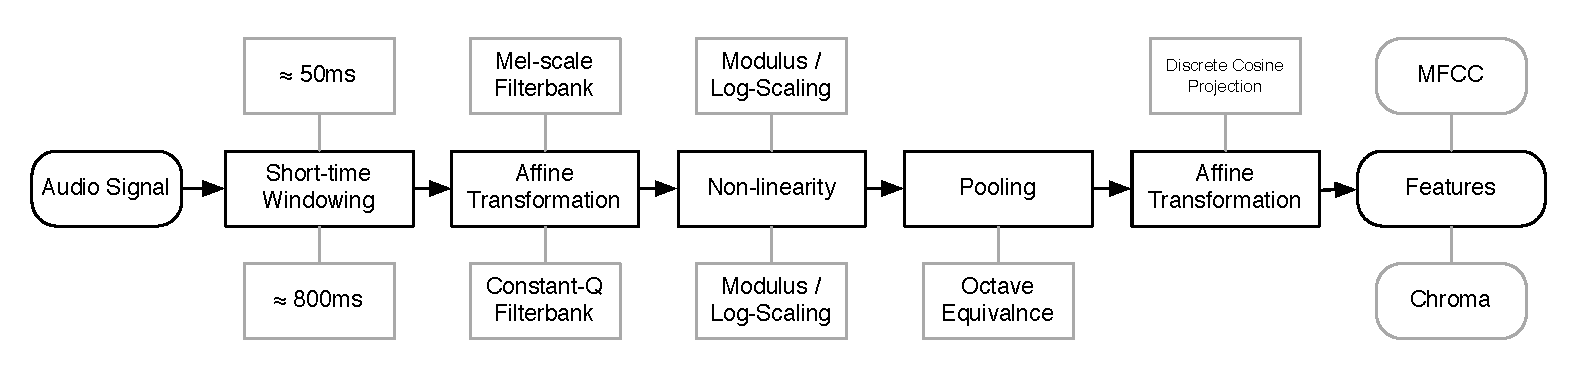
\includegraphics[width=\textwidth]{simplearch}
\caption{\emph{State of the art}: Standard approaches to feature extraction proceed as the cascaded combination of a few simpler operations; on closer inspection, the main difference between chroma and MFCCs is the parameters used.}
\label{fig:simplearch}
\end{centering}
\end{figure}


Considering this formulation, there are three specific reasons why this approach might be problematic.
First, though the data-driven training of classifiers and other pattern recognition machines has been standard for over a decade in music informatics, the parametrization of feature extractors ---e.g. choice of filters, non-linearities and pooling strategies, and the order in which they are applied--- remains, by and large, a manual process.
Both feature extraction and classifier training present the same basic problem: there is a large solution space and, somewhere in it, a configuration that optimizes an objective function over a dataset.
Though the music informatics community is privileged with a handful of talented researchers who are particularly adept at exploring this daunting space, crafting good features can be a time consuming and non-trivial task.
Additionally, carefully tuning features for one specific application offers no guarantees about relevance or versatility in another scenario.
As a result, features developed for one task ---chroma for chord recognition \cite{Fujishima1999} or MFCCs in speech \cite{Mermelstein1980}--- are used in others they were not specifically designed for, e.g. structural segmentation \cite{Levy2007} or music classification \cite{Mandel2005}.
The caveat of repurposing features designed for other applications is that, despite potentially giving encouraging results, they are not optimized for this new use case.
In fact, recent research has demonstrated that better features than MFCCs exist for \emph{speech recognition} \cite{Hinton2012}, the very task they were designed for, so it is almost certain that there are better musical features as well.
Therefore, the conclusions to draw from this are twofold: continuing to manually optimize a feature representation is not scalable to every problem, and we may be unnecessarily constraining our search of the solution space.


Second, these information processing architectures can be said to be \emph{shallow}, i.e. incorporating only a few non-linear transformations in their processing chain.
Sound, like other real-world phenomena, naturally lives on a highly non-linear manifold within its time-domain representation.
Shallow processing structures are placed under a great deal of pressure to accurately characterize the latent complexity of this data.
Feature extraction can thusly be conceptualized as a function that maps inputs to outputs with an order determined by its \emph{depth}; for a comprehensive discussion on the merits and mathematics of depth, we refer the curious reader to \cite{Bengio2009}.
Consider the example in Figure \ref{fig:curvefit}, where the goal is to compute a low-dimensional feature vector (16 coefficients) that describes the log-magnitude spectrum of a windowed violin signal.
One possible solution to this problem is to use a \emph{channel vocoder} which, simply put, low-pass filters and decimates the spectrum, producing a piece-wise linear approximation of the envelope.
It is clear, however, that with only a few linear components we cannot accurately model the latent complexity of the data, obtaining instead a coarse approximation.
Alternatively, the \emph{cepstrum} method transforms the log-magnitude spectrum before low-pass filtering.
In this case, the increase in depth allows the same number of coefficients to more accurately represent the envelope.
Obviously, powerful pattern recognition machines can be used in an effort to compensate for the deficiencies of a feature representation.
However, shallow, low-order functions are fundamentally limited in the kinds of behavior they can characterize, and this is problematic when the complexity of the data greatly exceeds the complexity of the model.

\begin{figure}[t]
\begin{centering}
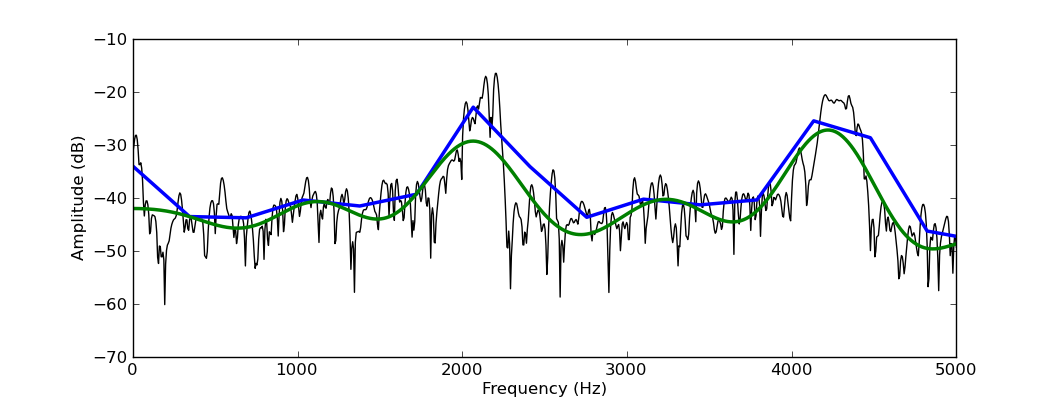
\includegraphics[height=1.5 in]{specfit}
\caption{\emph{Low-order approximations of highly non-linear data}: The log-magnitude spectra of a violin signal (black) is characterized by a channel vocoder (blue) and cepstrum coefficients (green). The latter, being a higher-order function, is able to more accurately describe the contour with the same number of coefficients.}
\label{fig:curvefit}
\end{centering}
\end{figure}

Third, short-time signal analysis is intuitively problematic because the vast majority of our musical experiences do not live in hundred millisecond intervals, but at least on the order of seconds or minutes.
Conventionally, features derived from short-time signals are limited to the information content contained within each segment.
As a result, if some musical event does not occur within the span of an observation ---a motif that does not fit within a single frame--- then it simply cannot be described by that feature vector alone.
This is clearly an obstacle to capturing high-level information that unfolds over longer durations, noting that time is extremely, if not fundamentally, important to how music is perceived.
Admittedly, it is not immediately obvious how to incorporate longer, or even multiple, time scales into a feature representation, with previous efforts often taking one of a few simple forms.
\emph{Shingling} is one such approach, where a consecutive series of features is concatenated into a single, high-dimensional vector \cite{Casey2008}.
In practice, shingling can be fragile to even slight translations that may arise from tempo or pitch modulations.
Alternatively, \emph{bag-of-frames (BoF)} models consider patches of features, fitting the observations to a probability distribution.
As addressed earlier with Figure \ref{fig:mfccs}, bagging features discards temporal structure, such that any permutation of the feature sequence yields the same distribution.
The most straightforward technique is to ignore longer time scales at the feature level altogether, relying on post-filtering \emph{after} classification to produce more musically plausible results.
For this to be effective though, the musical object of interest must live at the time-scale of the feature vector or it cannot truly be encoded.
Ultimately, none of these approaches are well suited to characterizing structure over musically meaningful time-scales.



\section{A Concise Summary of Current Obstacles}
\label{sec:obstacles}
In an effort to understand why progress in content-based music informatics is plateauing, we have reviewed the standard approach to music signal processing and feature design, deconstructing assumptions and motivations behind various decisions.
As a result, three potential areas of improvement are identified.
So that each may be addressed in turn, it is useful to succinctly restate the main points of this section:

\begin{itemize}

\item \textbf{Hand-crafted feature design is neither scalable nor sustainable}: Framing feature design as a search in a solution space, the goal is to discover the configuration that optimizes an objective function. Even conceding that some gifted researchers might be able to achieve this on their own, they are too few and the process too time-consuming to realistically solve every feature design challenge that will arise. \\
\item \textbf{Shallow processing architectures struggle to describe the latent complexity of real-world phenomena}: Feature extraction is similar in principle to compactly approximating functions. Real data, however, lives on a highly non-linear manifold and shallow, low-order functions have difficulty describing this information accurately. \\
\item \textbf{Short-time analysis cannot naturally capture higher level information}: Despite the importance of long-term structure in music, features are predominantly derived from short-time segments. These statistics cannot capture information beyond the scope of its observation, and common approaches to characterizing longer time scales are ill-suited to music.\\

\end{itemize}


\section{Deeper Architectures in MIR}
While many current systems rely on low-level, hand-crafted feature extraction and the subsequent interpretation by powerful machine learning algorithms, some in the community have begun to embrace different extensions to these approaches.
Research in automatic music feature learning began with the research of Pachet and Cabral with the EDS system, designed to find the optimal configuration of processing elements to yield the best features for different applications, such as music description or chord recognition \cite{Pachet2003, Pachet2006}.
In a similar vein, sparse mid-level representations have been explored for timbre recognition, where a dictionary of acoustic basis functions---sound atoms---are learned from music signals \cite{Richard2006}.
Moving away from shallow, short-time statistics, some have started to explore hierarchical filterbanks \cite{Anden2011} and multi-scale representations \cite{Hamel2011, Hamel2012} to characterize longer duration signals.

There are instances where deep signal processing structures have evolved naturally in the course of ongoing research, and there is one worth illustrating here.
State of the art tempo estimation algorithms have, for some time now, been based on deep, non-linear processing architectures.
The high-level intuition behind system design is relatively straightforward and, as evidenced by various approaches, widely agreed upon; first identify the occurrence of musical events, or onsets, and then estimate the underlying periodicity.
The earliest efforts in tempo analysis tracked symbolic events \cite{Dannenberg1984}, but it was soon shown that a time-frequency representation was advantageous in encoding rhythmic information \cite{Scheirer1998}.
This led to in-depth studies of onset detection \cite{Bello2005}, based on the idea that ``good'' impulse-like signals, referred to as \emph{novelty functions}, would greatly simplify periodicity analysis.
Along the way, it was also discovered that applying non-linear compression to a novelty function produced noticeably better results \cite{Klapuri2006}.
Various periodicity tracking methods were simultaneously explored, including oscillators \cite{Large1994}, multiple agents \cite{Goto1995}, inter-onset interval histograms \cite{Dixon2007}, and tuned filterbanks \cite{Grosche2011}.

\begin{figure}
\begin{centering}
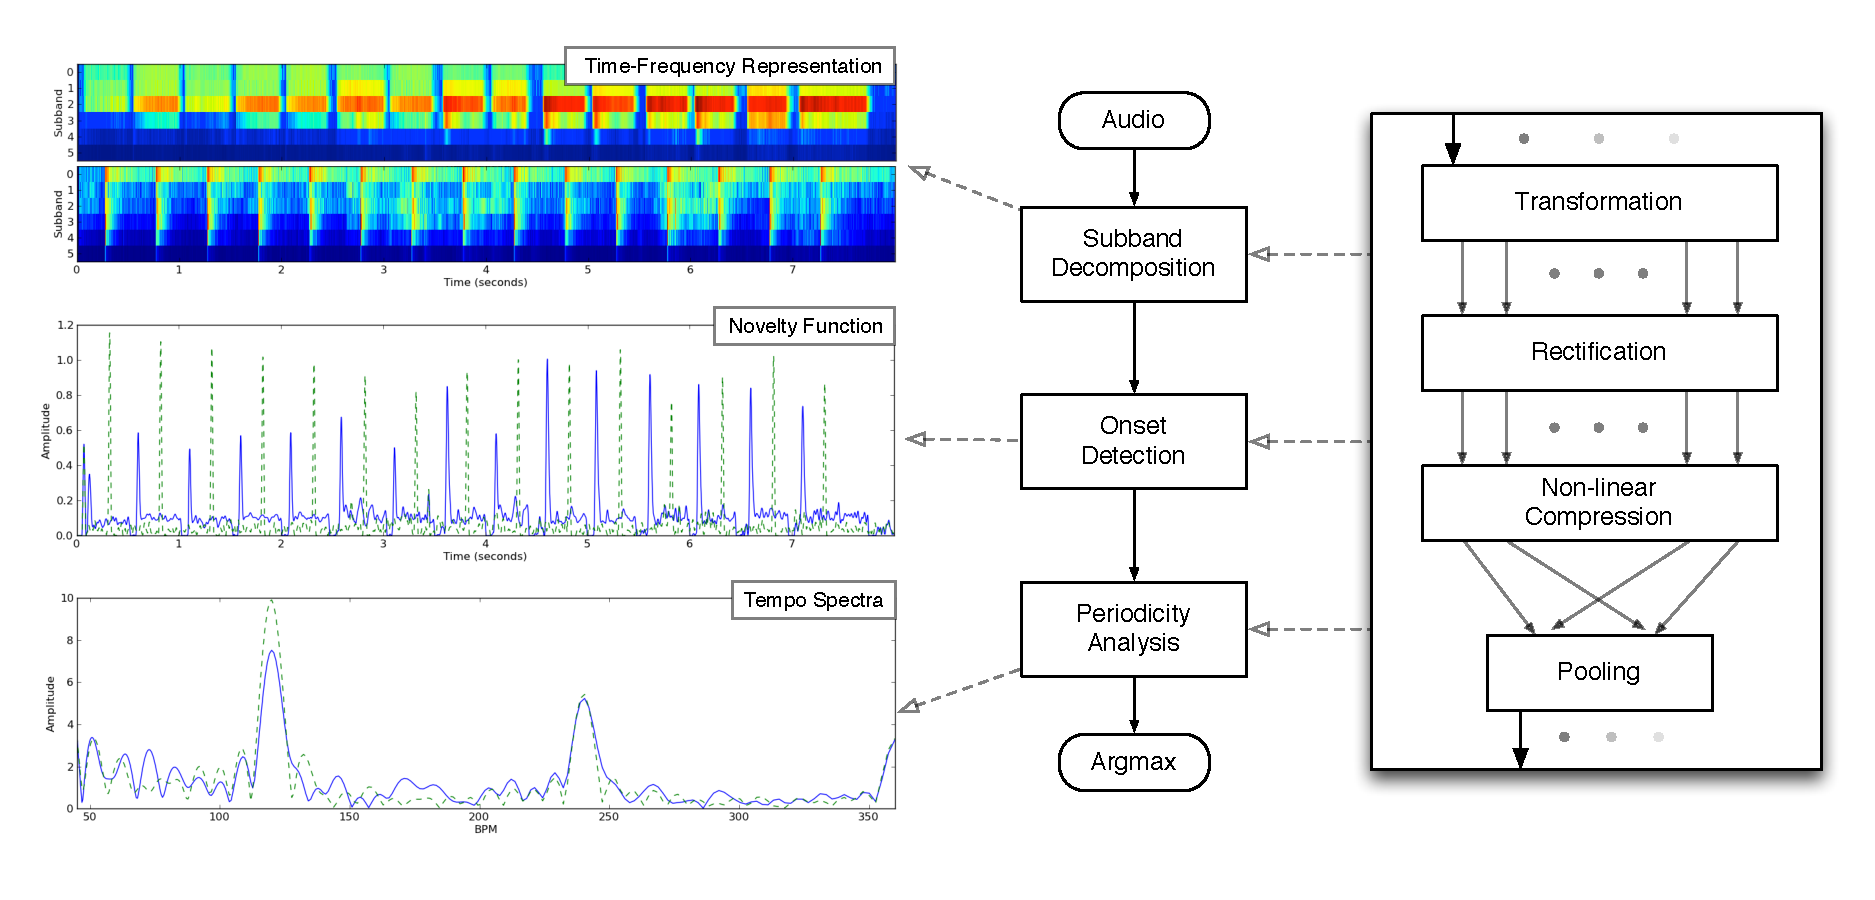
\includegraphics[width=\textwidth]{hierarchicaltecture}
\caption{\emph{A complex system of simple parts}: Tempo estimation has, over time, naturally converged to a deep architecture with strong parallels to a CNN. Note how each processing layer absorbs a different type of variance ---absolute amplitude, pitch and timbre, and phase--- to transform two different signals into nearly identical representations.}
\label{fig:deeparchs}
\end{centering}
\end{figure}

Reflecting on this lineage, system design has, over time, effectively converged to a deep learning architecture, minus the learning, where the same processing elements ---filtering and transforms, non-linearities, and pooling--- are replicated over multiple processing layers.
Interestingly, as shown in Figure \ref{fig:deeparchs}, visual inspection demonstrates why it is particularly well suited to the task of tempo estimation.
Here we consider two input waveforms having nothing in common but tempo; one is an ascending D Major scale played on a trumpet, and the other is a delayed series of bass drum hits.
It can be seen that, at each layer, a different kind of variance in the signal is removed.
The filterbank front-end absorbs rapid fluctuations in the time-domain signal, spectrally separating acoustic events.
This facilitates onset detection, which provides a pitch and timbre invariant estimate of events in the signal, reducing information along the frequency dimension.
Lastly, periodicity analysis eliminates shifts in the pulse train by discarding phase information.
At the output of the system, these two acoustically different inputs have been transformed into nearly identical representations.
Therefore, the most important lesson demonstrated by this example is how invariance can be achieved by distributing complexity over multiple processing layers.

This realization is beginning to spread throughout the MIR community, and there is, understandably, an increasing interest in the application of deep learning methods to these problems.
Among the first uses of deep learning were the application of CNNs to the detection of onsets \cite{Lacoste2007} and long short-term memory to model symbolic music sequences \cite{Eck2008}.
Deep Belief Networks quickly gained popularity for genre recognition \cite{Hamel2009}, mood estimation \cite{Schmidt2011}, note transcription \cite{Nam2011}, and artist recognition \cite{Dieleman2011}, but somewhat surprisingly many of these methods operate on single, short-time observations of the music signal.
Incorporating longer time-scales, CNNs have also been used to classify inputs on the order of seconds for, again, genre recognition \cite{Li2010}, instrument classification \cite{Humphrey2010} and chord recognition \cite{Humphrey2011, Humphrey2012b}.
Predictive Sparse Decomposition (PSD) and methods inspired by sparse coding have also seen a spike in activity over the last two years for a variety of tasks \cite{Henaff2011, Nam2012}, but despite being developed for deep learning, neither of these systems are actually hierarchical.

% It is worthwhile to note that many, if not all, of these works have achieved state of the art performance on their respective tasks, often in the first application of the method to the area.
% Any instances where this has occurred, however, deep learning techniques have simply been directly some kind of derived audio representation with minimal modification.
% It is therefore important to realize that these methods have never been tailored to address the nuances of music signals, and more importantly time.
% Overall, only CNNs make an effort to consider observations on the order of seconds, but do so in an admittedly awkward way, requiring the observation length be defined \emph{a priori}.
% The machine is ultimately limited to the amount of information it sees in its analysis, and there is obviously no fixed duration in which all musical behavior resides.
